\section{Pêndulo Simples}

O pêndulo simples é um sistema teórico composto por uma esfera de massa $m$ suportada por uma corda fina ou fio de massa desprezível. Tal sistema é um exemplo de um movimento harmônico simples.

O movimento de um pêndulo oscilante é estudado fazendo se as devidas considerações que simplificam essa análise.

\begin{figure}[H]
	\centering
	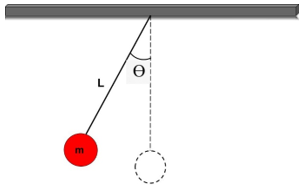
\includegraphics[width=0.8\textwidth]{./Imagens/Pendulo simples/ps1.png} 
	\caption{Sistema pêndulo simples}
	\label{fig:PS1}
\end{figure}

Este movimento pode ser descrito pela seguinte expressão:

$$\Large \frac{d^2\theta}{dt^2} + \frac{g}{L}sen(\theta) = 0$$

Onde $\theta$ representa o ângulo de deslocamento da esfera em relação a posição de equilíbrio na vertical, $t$  o tempo, $g$ a aceleração da gravidade e $L$ o comprimento do fio.

Temos aqui uma equação diferencial ordinária de 2ª ordem de resolução analítica relativamente complexa.

Para simplificação da resolução é feita a seguinte aproximação: para ângulos pequenos ($\theta \ll 1$),  $sen(\theta)  \approx  \theta$.  A equação se torna então: 

$$\Large \frac{d^2\theta}{dt^2} + \frac{g}{L}\theta = 0$$

Entretanto tem – se um desvio considerado do comportamento real desse sistema aplicando – se essa simplificação. Para contornar isso, podemos recorrer a métodos numéricos que fornecem com precisão satisfatória a resolução da equação original (sem a simplificação) supracitada.

Para isso vamos utilizar o software Scilab e sua linguagem para resolver essa EDO de 2ª ordem. Aplicaremos o método de Euler que consiste em um dos métodos de passo único no que tange a resolução de equações diferenciais ordinárias. Antes de tudo temos que transformar essa equação de 2ª ordem em um sistema com duas equações de 1ª ordem. Chamamos a $\large \frac{d\theta(t)}{dt} = \omega$, assim, por consequência temos que a derivada segunda de $\theta$ é igual a $\large \frac{d^2\theta}{dt^2} = \frac{d\omega}{dt}$ sendo assim podemos substituir tais termos na equação 4, resultando no seguinte sistema:

$$\Large \frac{d\theta(t)}{dt} = \omega$$

$$\Large \frac{d\omega}{dt} = -\frac{g}{L} sen(\theta(t))$$

Sendo assim, aplicamos o método de Euler no sistema para determinar o comportamento de $\theta(t)$ em relação ao tempo:

\begin{minted}{Scilab}
// resolução de sistema de 2 equações representando 
// o movimento de um pêndulo simples
clear,clc
// definindo o intervalo de tempo
t0 = input("informe o valor inicial do intervalo: ");
tn = input("informe o valor final do intervalo: ");
h = input("Informe o passo h: ");
t = t0:h:tn // criando o vetor intervalo de tempo
t = t' // apenas transpoe o vetor t

L = input("informe o comprimento do fio")
g= 9.8 //aceleração da gravidade

//condições iniciais
w1(1) = 0.785398163 // 45 graus em radianos
w2(1) = 0
for j = 2:length(t)
w1(j) = w1(j-1) + w2(j-1)*h
w2(j) = w2(j-1) -(g/L)*sin(w1(j-1))*h
end

//solução linear 
function y = f(t)
y = 0.785398163*cos(sqrt(g/L)*t)
endfunction

plot(t,w2,'b', t, f, 'r')
legends(["Não Linear", "Linear"], opt = "lr")
\end{minted}